\documentclass[a4paper,12pt,titlepage]{article}
\usepackage{fullpage}
\usepackage[utf8]{inputenc}
\usepackage[francais]{babel}
\usepackage[T1]{fontenc}
\usepackage{graphicx}
\usepackage{amsmath}
\usepackage{amssymb}
%\usepackage{fourier-orns} % panneau danger
%\usepackage{mathrsfs}
\begin{document}
	
		
	 
	{\hfill 
\includegraphics[scale=0.15]{LogoENSSAT.jpg}}\\
	Gaudillat Valentine \\ 

    
    
	\begin{verbatim}
	
	
	
	
	
	

	

	\end{verbatim}
	{\centering \section*{Compte Rendu ONL2 :} \section*{Instabilite de modulation}}
	\begin{verbatim}
	
	
	
	
	\end{verbatim}
	
	\begin{center}
		%\includegraphics[scale=0.3]{}
	\end{center}
	%\begin{verbatim}
		
		
		
		
		
		
		
		
		
		
		
		
	%\end{verbatim}
	
	\clearpage
	\tableofcontents 
	\newpage
    
    
    \section{Introduction :}
        Lorsque une impulsion lumineuse traverse un milieu non linéaire d'ordre 3, un processus de mélange à quatre ondes peut intervenir. Il peut en résulter une instabilité de modulation. 
        
        ~\\~
        
        Soit un faisceau incident, monochromatique ($\omega_{p}$), à la puissance moyenne P$_0$. Le champ est modulé à $\Omega$. On appelle $\delta$ la profondeur de modulation. 
        
        On le propage dans une fibre optique d'aire effective $A_{eff} = \frac{d_eff}{2}^2$, de coefficient non linéaire $\gamma$ (W$^{-1}$m$^{-1}$) et de dispersion de vitesse de groupe $\beta_2$ (s$^2$m$^{-1}$).
        
        ~\\~
        
        On écrit l'enveloppe du champ en z comme :
        
        \begin{equation}
        A(z,t) = \sqrt{\frac{P_{0}}{2n\epsilon_0cA_{eff}}}(1+\delta(z) cos(\Omega t))
        \end{equation}
        
        Si et seulement si $\Omega$ < $\Omega_c$ tel que : 
        
        \begin{equation*}
            \Omega_c = \sqrt{\frac{4\gamma P_0}{|\beta_2|}}
        \end{equation*}
        
        Alors, \\
        {\centering $\delta(z) = \delta(0) \text{e}^{gz}$.\\}
        Avec $g(\Omega,P_0) = \frac{|\beta_2|\Omega}{2}\sqrt{\Omega_c^2 - \Omega^2}$
        
        
        ~\\~
        
        On prend les valeurs numériques suivantes :
        
        \begin{itemize}
            \item c =$ 3*10^8 $                    Célérité de la lumière (m s$^{-1}$)
            \item $\epsilon_0 = 8.85 * 10^{-12}$ :   Permittivité du vide (F m$^{-1}$)
            \item $\beta_2 = -2 * 10^{-26}$ :       Dispersion de vitesse de groupe (s$^2$m$^{-1}$)
            \item $\gamma = 2*10^{-3}$ :            Coefficient non linéaire (W$^{-1}$m$^{-1}$)
            \item $d_{eff} = 10*10^{-6}$ :           Diamètre effectif du mode guidé (m)
            \item $A_{eff} = \pi*(d_{eff}/2)^2$ :       Aire effective (m$^2$)
            \item $n = 1.47$ :                     Indice de réfraction
            \item $\lambda_p = 532 * 10^{-9}$ :    Longueur d'onde du faisceau (m)
            \item $\delta_0 = 0.02$ :              Profondeur de modulation initiale
        \end{itemize}
        
    \newpage
    
    \section{Évolution du gain linéique en fonction de la fréquence de modulation}
    
    \begin{figure}
        \centering
        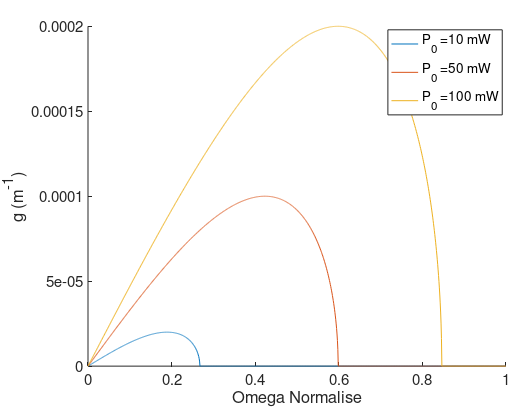
\includegraphics{g(omega)}
        \caption{Évolution du gain linéique en fonction de la fréquence de modulation}
        \label{delta}
    \end{figure}
    
    
    \newpage
    
    \section{Évolution }
    
    \begin{figure}
        \centering
        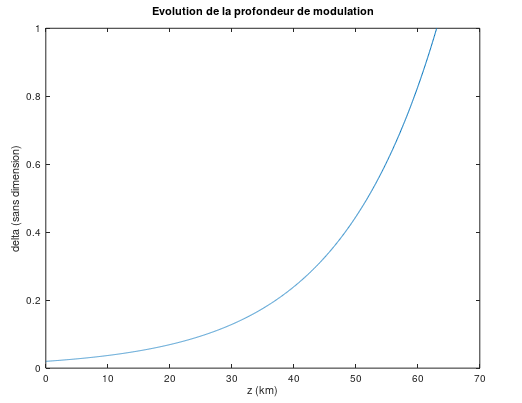
\includegraphics{delta(z)}
        \caption{Évolution de la profondeur de modulation en fonction de la longueur de fibre étudiée}
        \label{delta}
    \end{figure}
    
\end{document}
